\documentclass[12pt, a4paper]{article}
\usepackage{../../../myconfig} % Gọi file cấu hình từ ngoài gốc vào

% ==========================================
% BẮT ĐẦU NỘI DUNG TÀI LIỆU
% ==========================================
\begin{document}

% Truyền 3 tham số: {Nhãn cam} {Chữ to chính giữa} {Chữ ở góc phải Header}
\titlebox{Chủ đề: Hàm số}{BTDD hàm số hữu tỉ}{Hàm số: Hàm hữu tỉ}

\questionLinesManual{0}{1}{Hàm số nào dưới đây có đồ thị như hình vẽ sau?

\begin{center}
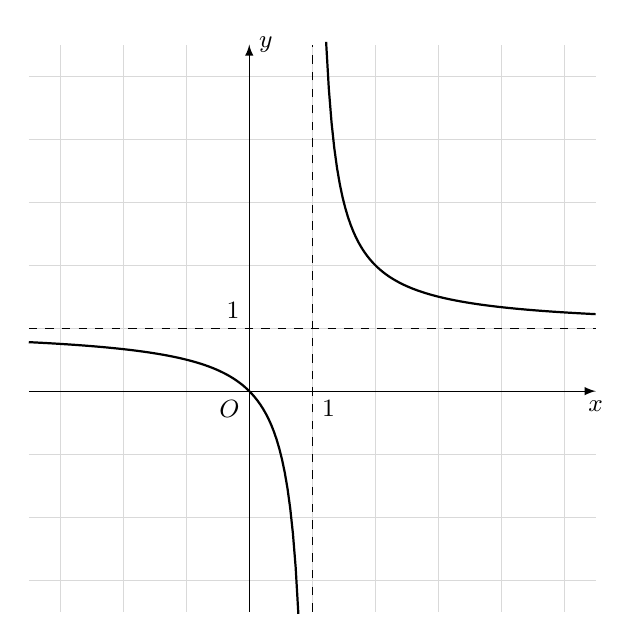
\begin{tikzpicture}[>=latex, scale=0.8]
    % 1. Vẽ lưới
    \draw[color=gray!30, thin, step=1] (-3.5,-3.5) grid (5.5,5.5);
    
    % 2. Vẽ hệ trục tọa độ
    \draw[->] (-3.5,0) -- (5.5,0) node[below] {\small $x$};
    \draw[->] (0,-3.5) -- (0,5.5) node[right] {\small $y$};
    \node[below left] at (0,0) {\small $O$};
    
    % 4. Vẽ đồ thị hàm số y = x/(x-1)
    \draw[thick, samples=100, domain=-3.5:0.78] 
        plot (\x, {\x/(\x - 1)});
    \draw[thick, samples=100, domain=1.22:5.5] 
        plot (\x, {\x/(\x - 1)});
    
    % 5. Đường tiệm cận
    \draw[dashed] (1,-3.5) -- (1,5.5);
    \draw[dashed] (-3.5,1) -- (5.5,1) ;
    \node[below right] at ( 1,0) {\small $1$};
    \node [ above left] at (0,1) {\small $1$};
\end{tikzpicture}
\end{center}

}{
    \begin{tasks}(4)
        \task \( y = \dfrac{x}{x+1} \)
        \task \( y = -\dfrac{x}{x-1} \)
        \task \( y = -\dfrac{x}{x+1} \)
        \task \( y = \dfrac{x}{x-1} \)
    \end{tasks}
}

\questionLinesManual{0}{2}{Đường cong ở hình dưới đây là đồ thị của hàm số

\begin{center}
\begin{tikzpicture}[>=latex, scale=0.6]
    \draw[->] (-3.5,0) -- (4.5,0) node[below] {\small $x$};
    \draw[->] (0,-3.5) -- (0,5.5) node[right] {\small $y$};
    \node[below right] at (0,0) {\tiny $O$};
    
    % 3. Đánh dấu các mốc
    \foreach \x in {-3,-2,1,2,3,4} {
        \draw (\x,0.05) -- (\x,-0.05) node[below] {\tiny $\x$};
    }
    \foreach \val in {-3,-2,-1,1,2,3} {
        \draw (0.05,\val) -- (-0.05,\val) node[left] {\tiny $\val$};
    }
    
    % 4. Vẽ đồ thị hàm số y = (x^2 - x + 1)/(x - 1)
    \draw[thick, samples=100, domain=-3.5:0.76] 
        plot (\x, {(\x*\x - \x + 1)/(\x - 1)});
    \draw[thick, samples=100, domain=1.23:5.5] 
        plot (\x, {(\x*\x - \x + 1)/(\x - 1)});
    
    % 5. Đường tiệm cận
    \draw[dashed] (1,5.5) -- (1,-3.5) node[below] {\small $x=1$};
    \draw[dashed] (-3.5,-3.5) -- (5.5,5.5) node[ below right] {\small $y=x$};
\end{tikzpicture}
\end{center}

}{
    \begin{tasks}(4)
        \task \( y = \dfrac{x^2 - 4x + 5}{x - 2} \)
        \task \( y = \dfrac{x^2 - 4x - 1}{x + 1} \)
        \task \( y = \dfrac{x^2 - x + 1}{x - 1} \)
        \task \( y = \dfrac{x^2 + x - 1}{x - 1} \)
    \end{tasks}
}

\questionLinesManual{0}{3}{Cho hàm số \( y = \dfrac{ax + b}{cx + d} \) (\(a, b, c \in \mathbb{R}\)) có đồ thị là đường cong như hình vẽ bên:

\begin{center}
\begin{tikzpicture}[>=latex, scale=0.8]
    % 1. Hệ trục tọa độ
    \draw[->] (-4.5,0) -- (3.5,0) node[below] {\small $x$};
    \draw[->] (0,-3.5) -- (0,4.5) node[right] {\small $y$};
    \node[below left] at (0,0) {\small $O$};
    % 3. Vẽ đồ thị hàm số y = (x+1)/(x-1)
    \draw[thick, samples=100, domain=-4.5:-1.56] 
        plot (\x, {(\x - 1)/(\x + 1)});
    \draw[thick, samples=100, domain=-0.56:3.5] 
        plot (\x, {(\x - 1)/(\x +1)});
    
    % 4. Đường tiệm cận
    \draw[dashed] (-1,-3.5) -- (-1,4.5);
    \draw[dashed] (-4.5,1) -- (3.5,1);
    
    \node[below left] at (-1,0) {\small $-1$};
    \node [above left] at ( 0,1) {\small $1$};
\end{tikzpicture}
\end{center}

Toạ độ tâm đối xứng của đồ thị hàm số đã cho là:}{
    \begin{tasks}(4)
        \task \((-1; 1)\)
        \task \((1; 1)\)
        \task \((1; -1)\)
        \task \((0; 1)\)
    \end{tasks}
}

\questionLinesManual{0}{4}{Đường cong như hình vẽ dưới đây là đồ thị của hàm số nào?

\begin{center}
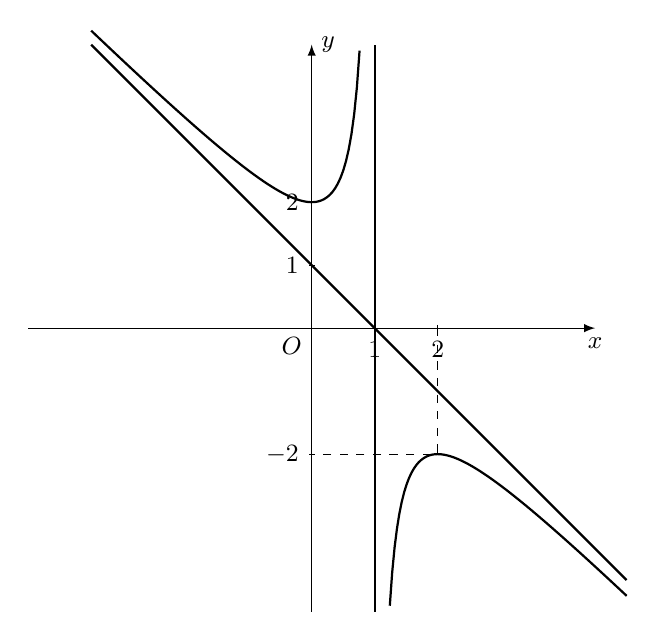
\begin{tikzpicture}[>=latex, scale=0.8]
    % 1. Hệ trục tọa độ
    \draw[->] (-4.5,0) -- (4.5,0) node[below] {\small $x$};
    \draw[->] (0,-4.5) -- (0,4.5) node[right] {\small $y$};
    \node[below left] at (0,0) {\small $O$};
    
    % 2. Đánh dấu các mốc
    \foreach \x in {1,2} {
        \draw (\x,0.05) -- (\x,-0.05) node[below] {\small $\x$};
    }
    \foreach \val in {-2,1,2} {
        \draw (0.05,\val) -- (-0.05,\val) node[left] {\small $\val$};
    }
    
    % 3. Vẽ đồ thị hàm số y = (-x^2 + 2x - 2)/(x-1)
    \draw[thick, samples=100, domain=-3.5:0.76] 
        plot (\x, {(-\x*\x + 2*\x - 2)/(\x - 1)});
    \draw[thick, samples=100, domain=1.24:5] 
        plot (\x, {(-\x*\x + 2*\x - 2)/(\x - 1)});
     \draw[thick, samples=100, domain=-3.5:5] 
        plot (\x, {(-\x+1});
    % 4. Đường tiệm cận
    \draw[thick] (1,-4.5) -- (1,4.5);
    \draw [dashed] (2,0) -- ( 2,-2) -- ( 0,-2);
\end{tikzpicture}
\end{center}

}{
    \begin{tasks}(4)
        \task \( y = \dfrac{x-2}{x-1} \)
        \task \( y = \dfrac{x^2 + 2x - 2}{x-1} \)
        \task \( y = \dfrac{-x^2 + 2x - 2}{x-1} \)
        \task \( y = \dfrac{-x^2 + x - 2}{x-1} \)
    \end{tasks}
}

\questionLinesManual{0}{5}{Hình vẽ bên là đồ thị hàm số \( y = \dfrac{ax + b}{cx + d} \). Mệnh đề nào dưới đây đúng?

\begin{center}
\begin{tikzpicture}[>=latex, scale=0.8]
    % Vẽ hệ trục
    \draw[->] (-5.5,0) -- (3.5,0) node[below] {$x$};
    \draw[->] (0,-3.5) -- (0,5.5) node[right] {$y$};
    \node[below left] at (0,0) {$O$};
    
    % Vẽ đồ thị hàm số
    \draw[thick, samples=100, domain=-5.5:-1.33] 
        plot (\x, {(\x - 0.5)/(\x + 1)});
    \draw[thick, samples=100, domain=-0.67:3.5] 
        plot (\x, {(\x - 0.5)/(\x + 1)});
    
    % Đường tiệm cận
    \draw[dashed] (-1,-3.5) -- (-1,5.5);
    \draw[dashed] (-5.5,1) -- (3.5,1);
\end{tikzpicture}
\end{center}

}{
    \begin{tasks}(4)
        \task \( ad > 0 \) và \( bd > 0 \)
        \task \( ad > 0 \) và \( ab < 0 \)
        \task \( bd < 0 \) và \( ab > 0 \)
        \task \( ad < 0 \) và \( ab < 0 \)
    \end{tasks}
}

\questionLinesManual{0}{6}{Cho hàm số \( y = \dfrac{ax^2 + bx + c}{a'x + b'} \) (\(a>0, a' \neq 0 \))  có đồ thị như hình vẽ bên. Hàm số đã cho nghịch biến trên khoảng nào trong các khoảng sau đây?

\begin{center}
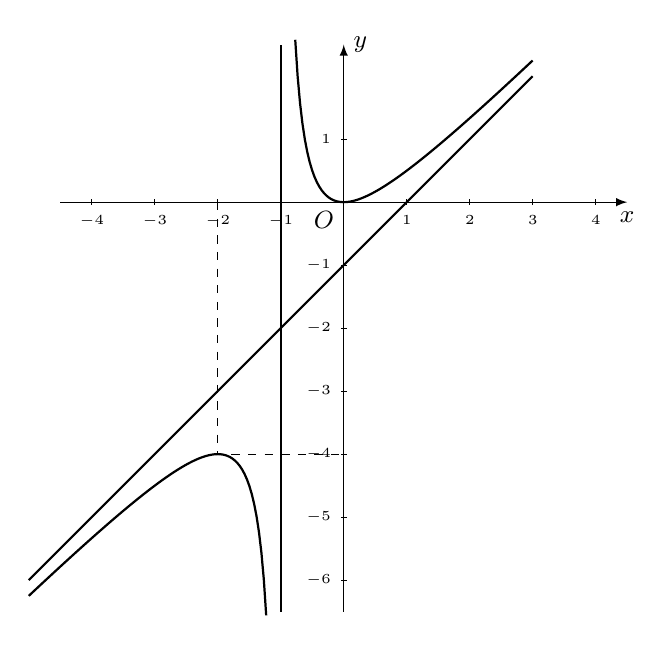
\begin{tikzpicture}[>=latex, scale=0.8]
    % 1. Hệ trục tọa độ
    \draw[->] (-4.5,0) -- (4.5,0) node[below] {\small $x$};
    \draw[->] (0,-6.5) -- (0,2.5) node[right] {\small $y$};
    \node[below left] at (0,0) {\small $O$};
    
    % 2. Đánh dấu các mốc
    \foreach \x in {-4,-3,-2,-1,1,2,3,4} {
        \draw (\x,0.05) -- (\x,-0.05) node[below] {\tiny $\x$};
    }
    \foreach \val in {,-6,-5,-4,-3,-2,-1,1,} {
        \draw (0.05,\val) -- (-0.05,\val) node[left] {\tiny $\val$};
    }
    
    % 3. Vẽ đồ thị hàm số y = (x^2 + 2x + 2)/(x + 1)
    \draw[thick, samples=100, domain=-5:-1.23] 
        plot (\x, {(\x*\x + 2*\x + 2)/(\x + 1)-2});
    \draw[thick, samples=100, domain=-0.77:3] 
        plot (\x, {(\x*\x + 2*\x + 2)/(\x + 1)-2});
    \draw[thick, samples=100, domain=-5:3] 
        plot (\x, {\x-1});
    \draw[dashed] (-2,0) -- (-2,-4) --(0,-4);
    % 4. Đường tiệm cận
    \draw[thick] (-1,-6.5) -- (-1,2.5);
\end{tikzpicture}
\end{center}

Trong các số \( b, c, a', b' \) có tất cả bao nhiêu số dương?}{
    \begin{tasks}(4)
        \task $1$
        \task $2$
        \task $3$
        \task $4$
    \end{tasks}
}

\questionLinesManual{0}{7}{Cho hàm số \( y = \dfrac{x^2 + 2x + 2}{x + 1} \). Tâm đối xứng của đồ thị hàm số là:}{
    \begin{tasks}(4)
        \task \( I(-1; 0) \)
        \task \( I(-1; 1) \)
        \task \( I(-1; 2) \)
        \task \( I(1; 1) \)
    \end{tasks}
}

\questionLinesManual{0}{8}{Đồ thị của hàm số \( y = \dfrac{x+1}{-x+1} \) là đường cong nào trong các hình vẽ sau?

\begin{center}

\end{center}

}{
    \begin{tasks}(2)
        \task \(
        \begin{tikzpicture}[>=latex, scale=0.8]
                % 1. Hệ trục tọa độ
                \draw[->] (-4.5,0) -- (3.5,0) node[below] {\small $x$};
                \draw[->] (0,-3.5) -- (0,4.5) node[right] {\small $y$};
                \node[below left] at (0,0) {\small $O$};
                
                % 2. Đánh dấu các mốc
                \foreach \x in {-1,1} {
                    \draw (\x,0.05) -- (\x,-0.05) node[below] {\small $\x$};
                }
                \foreach \val in {1} {
                    \draw (0.05,\val) -- (-0.05,\val) node[left] {\small $\val$};
                }
                
                % 3. Vẽ đồ thị hàm số y = (x+1)/(-x+1) = -(x+1)/(x-1)
                \draw[thick, samples=100, domain=-4.5:-1.57] 
                    plot (\x, {(\x - 1)/(\x + 1)});
                \draw[thick, samples=100, domain=-0.57:3.5] 
                    plot (\x, {(\x - 1)/(\x + 1)});
                
                % 4. Đường tiệm cận
                \draw[dashed] (-1,-3.5) -- (-1,4.5) ;
                \draw[dashed] (-4.5,1) -- (3.5,1) ;
            \end{tikzpicture}
        \)
        
        \task \(
        \begin{tikzpicture}[>=latex, scale=0.8]
                % 1. Hệ trục tọa độ
                \draw[->] (-3.5,0) -- (4.5,0) node[below] {\small $x$};
                \draw[->] (0,-4.5) -- (0,3.5) node[right] {\small $y$};
                \node[below left] at (0,0) {\small $O$};
                
                % 2. Đánh dấu các mốc
                \foreach \x in {-1,1} {
                    \draw (\x,0.05) -- (\x,-0.05) node[below] {\small $\x$};
                }
                \foreach \val in {-1,1} {
                    \draw (0.05,\val) -- (-0.05,\val) node[left] {\small $\val$};
                }
                
                % 3. Vẽ đồ thị hàm số y = (x+1)/(-x+1) = -(x+1)/(x-1)
                \draw[thick, samples=100, domain=-3.5:0.56] 
                    plot (\x, {(\x + 1)/(-\x + 1)});
                \draw[thick, samples=100, domain=1.57:4.5] 
                    plot (\x, {(\x + 1)/(-\x + 1)});
                
                % 4. Đường tiệm cận
                \draw[dashed] (1,-4.5) -- (1,3.5) ;
                \draw[dashed] (-3.5,-1) -- (4.5,-1) ;
            \end{tikzpicture}
        \)
        \task \(
        \begin{tikzpicture}[>=latex, scale=0.8]
                % 1. Hệ trục tọa độ
                \draw[->] (-4.5,0) -- (3.5,0) node[below] {\small $x$};
                \draw[->] (0,-4.5) -- (0,3.5) node[right] {\small $y$};
                \node[below left] at (0,0) {\small $O$};
                
                % 2. Đánh dấu các mốc
                \foreach \x in {-1,1} {
                    \draw (\x,0.05) -- (\x,-0.05) node[below] {\small $\x$};
                }
                \foreach \val in {-1,1} {
                    \draw (0.05,\val) -- (-0.05,\val) node[below left] {\small $\val$};
                }
                
                % 3. Vẽ đồ thị hàm số y = (x+1)/(-x+1) = -(x+1)/(x-1)
                \draw[thick, samples=100, domain=-4.5:-1.57] 
                    plot (\x, {(\x - 1)/(-\x - 1)});
                \draw[thick, samples=100, domain=-0.56:3.5] 
                    plot (\x, {(\x - 1)/(-\x - 1)});
                
                % 4. Đường tiệm cận
                \draw[dashed] (-1,-4.5) -- (-1,3.5);
                \draw[dashed] (-4.5,-1) -- (3.5,-1);
            \end{tikzpicture}
        \)
        \task \(
        \begin{tikzpicture}[>=latex, scale=0.8]
                % 1. Hệ trục tọa độ
                \draw[->] (-3.5,0) -- (4.5,0) node[below] {\small $x$};
                \draw[->] (0,-3.5) -- (0,4.5) node[right] {\small $y$};
                \node[below left] at (0,0) {\small $O$};
                
                % 2. Đánh dấu các mốc
                \foreach \x in {-1,1} {
                    \draw (\x,0.05) -- (\x,-0.05) node[below] {\small $\x$};
                }
                \foreach \val in {-1,1} {
                    \draw (0.05,\val) -- (-0.05,\val) node[left] {\small $\val$};
                }
                
                % 3. Vẽ đồ thị hàm số y = (x+1)/(-x+1) = -(x+1)/(x-1)
                \draw[thick, samples=100, domain=-3.5:0.56] 
                    plot (\x, {(\x + 1)/(\x - 1)});
                \draw[thick, samples=100, domain=1.57:4.5] 
                    plot (\x, {(\x + 1)/(\x - 1)});
                
                % 4. Đường tiệm cận
                \draw[dashed] (1,-3.5) -- (1,4.5) ;
                \draw[dashed] (-3.5,1) -- (4.5,1);
            \end{tikzpicture}
        \)
    \end{tasks}
}

\questionLinesManual{0}{9}{Phương trình tiếp tuyến của đồ thị hàm số \( y = \dfrac{x - 2}{x + 1} \) tại điểm có tung độ \(y_0 = -2\) là}{
    \begin{tasks}(4)
        \task \( y = 3x - 2 \)
        \task \( y = -3x + 2 \)
        \task \( y = 3x + 2 \)
        \task \( y = -3x - 2 \)
    \end{tasks}
}

\questionLinesManual{0}{10}{Cho hàm số \( y = \dfrac{ax + b}{x + c} \) có đồ thị như hình sau đây

\begin{center}
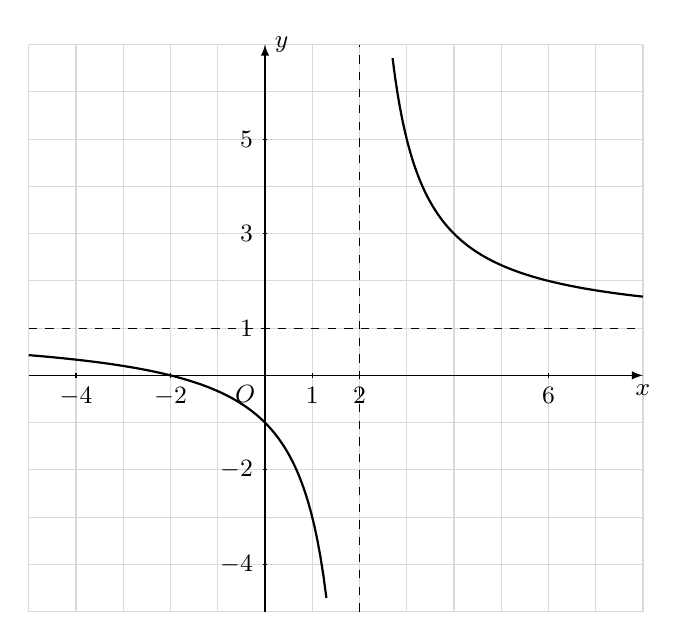
\begin{tikzpicture}[>=latex, scale=0.6]
    % 1. Vẽ lưới
    \draw[color=gray!30, thin, step=1] (-5,-5) grid (8,7);
    
    % 2. Vẽ hệ trục tọa độ
    \draw[->] (-5,0) -- (8,0) node[below] {\small $x$};
    \draw[->] (0,-5) -- (0,7) node[right] {\small $y$};
    \node[below left] at (0,0) {\small $O$};
    
    % 3. Đánh dấu các mốc
    \foreach \x in {-4,-2,1,2,6} {
        \draw (\x,0.05) -- (\x,-0.05) node[below] {\small $\x$};
    }
    \foreach \val in {-4,-2,1,3,5} {
        \draw (0.05,\val) -- (-0.05,\val) node[left] {\small $\val$};
    }
    
    % 4. Vẽ đồ thị hàm số y = (2x+1)/(x+1)
    \draw[thick, samples=100, domain=-5:1.3] 
        plot (\x, {(\x + 2)/(\x -2)});
    \draw[thick, samples=100, domain=2.7:8] 
        plot (\x, {(\x + 2)/(\x - 2)});
    
    % 5. Đường tiệm cận
    \draw[dashed] (2,-5) -- (2,7);
    \draw[dashed] (-5,1) -- (8,1);
\end{tikzpicture}
\end{center}

Tính giá trị của biểu thức \( P = 2a - b + 3c \).}{
    \begin{tasks}(4)
        \task $6$
        \task $-6$
        \task $10$
        \task $-2$
    \end{tasks}
}

\end{document}